\usetikzlibrary{trees,shadows}
\providecommand{\Energy}[1]{E_{#1}}
\providecommand{\pEnergy}[1]{E_{#1}}
\providecommand{\EnergyCol}{\Energy{col}}
\providecommand{\relp}[2]{\mathbf{p}_{#1}({#2})}
\providecommand{\dimsn}[1]{\mathbf{B}^{#1}}
\providecommand{\bb}[1]{d^{#1}(t)}
\providecommand{\trackpit}[2]{\mathbf{u}^{(#1)}(#2)}
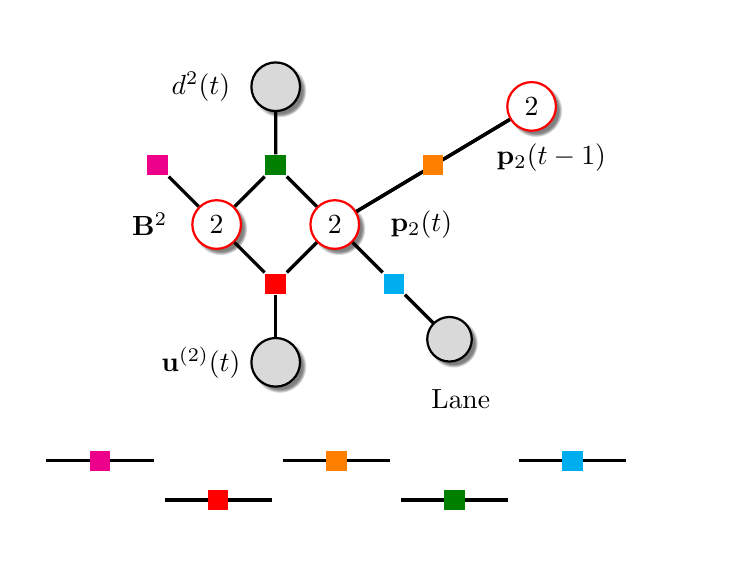
\begin{tikzpicture}[grow cyclic, line width=1.2,
    variablenode/.style={circle,circular drop shadow,draw=red,fill=white,thick,text=black},
    sizefactor/.style= {rectangle,inner sep=2,fill=magenta  ,thick,text=magenta},
    dynfactor/.style=  {rectangle,inner sep=2,fill=orange   ,thick,text=orange},
    lanefactor/.style= {rectangle,inner sep=2,fill=cyan    ,thick,text=cyan},
    trackfactor/.style={rectangle,inner sep=2,fill=red   ,thick,text=red},
    bboxfactor/.style= {rectangle,inner sep=2,fill=green!50!black,thick,text=green!50!black},
    level distance=30,
  obs/.style={fill=gray!30,text=gray!30,draw=black},
  prevf/.style={draw=green!20,text=gray},
  prevobsv/.style={draw=gray!10,fill=gray!1,text=gray},
  prevv/.style={draw=red!20,text=gray}
]
  \path[use as bounding box,clip] (-4.9, -4) rectangle (3.7,2.5);


  \path
  (-2.5,0) node[variablenode](dim) {2}
  +(-0.85, 0) node {$\dimsn{2}$}
  +(-0.75,0.75) node[sizefactor](fsize){\tiny{2}}
  ;

  \begin{scope}[line width=0.5]
    \path 
    % t-1 layer
    (1.5,1.5) node [variablenode] (xt1) {2}
    +(0.25, -0.65) node {$\relp{2}{t-1}$}
  %  [counterclockwise from=-100,sibling angle=60]
  %  +(1.0, -1.0) node [factor,prevf] (flane1) {$E_{lane}$} 
  %  child { node [variablenode,obs,prevobsv] (l1) { $L_t$ } }
  %  child { node [ variablenode,obs,font=\footnotesize,prevobsv] (gps1) {GPS}}
  %  child { node [ variablenode,obs,font=\footnotesize,prevobsv] (map1) {Map}}

  %  [counterclockwise from=220]
  %  +(-1.0, -1.0) node[factor,prevf](fpt1) {$E_{pt}$}
  %  child { node[variablenode,obs,prevobsv](pt1){$u_t$} }

  %  [counterclockwise from=60,sibling angle=60]
  %  +(-1, 1.0) node[factor,prevf](fdet1){$E_{det}$} 
  %   child {
  %     node[variablenode,obs,prevobsv](gp1){$G_t$} 
  %   }
  %   child { node[variablenode,obs,prevobsv](Det1){$D_t$}
  %   }

    ;

  %\draw [gray](xt1) -- (fdet1) -- (dim);
  %\draw [gray](xt1) -- (flane1);
  %\draw [gray](xt1) -- (fpt1);
      
  \end{scope}

   %(0.5,1.0) node [dynfactor] (fdynx) {}
  %(1.95,1.8) node [factor,draw=gray,text=gray,minimum width=3] (fdynt) {$E_{d}$}

 %(0.2,2.0) node[factor](fhol) {$E_{hol}$}

  %(1, 0)  node[variablenode](theta){$\theta_t$}
  \draw
  (-1, 0)  node[variablenode](xt) {2}
  + (1.10, 0) node {$\relp{2}{t}$}
  ++ (0.75, -0.75) node [lanefactor] (flane) {\tiny{2}} ;
%--
   %+ (-10:1) node [variablenode,obs] (l) {2} 
   % +(-10:1.8) node { $L_t$ } ;
\draw (flane) --
 + (-45:1) node [ variablenode,obs,font=\footnotesize] (gps) {2} +(-60:1.7) node {Lane};
%\draw (flane) -- +(-110:1)node [ variablenode,obs,font=\footnotesize] (map) {2} +(-110:1.7) node {Map};
 \path 
  (-1.75, .75) node[bboxfactor](fdet){\tiny{2}} 
  (-1.75, -.75) node[trackfactor] (fpt) {\tiny{2}};

 %++(65:1) node[variablenode,obs](gp){2} +(.75,0) node {$G_t$} ;
\draw (fdet)
--
++(90:1) node[variablenode,obs](Det){2} +(-.95,0) node {$\bb{2}$};
  
\draw (fpt) 
++(-90:1) node[variablenode,obs](pt){2} +(-.95,0) node {$\trackpit{2}{t}$} 
  ;
  \draw (xt) edge node [dynfactor] (fdynx) {\tiny{2}} (xt1);
  \draw (xt) -- (fdet) -- (Det);
  \draw (xt) -- (fpt) -- (dim);
  \draw (fpt) -- (pt);
  %\path  (fpt) edge (theta);
  %\draw (fdet) -- (gp);
 %(0.2,2.0) node[factor](fhol) {$E_{hol}$}
  %\draw (xt) edge [bend left=40] node[factor] (fhol) {$E_{hol}$} (xt1);
  %\draw (fhol) -- (theta);  	  
  \draw (dim) -- (fdet);
  \draw (fsize) -- (dim);
  %\draw (theta) -- (flane);
  \draw (xt) -- (fdynx) -- (xt1);
  %\draw (theta) -- (fdynt) -- (theta1);
  \draw (xt) -- (flane);
\coordinate (oneR) at (1.5,0);
  % Legend
  \path (-4.8, -3.0) node (ls) {}
  ++(oneR) node [anchor=west] (e1e) {$\EnergySize$}
  ++(oneR) node [] (e2s) {}
  ++(oneR) node [anchor=west] (e2e) {$\EnergyDyn$}
  ++(oneR) node [] (e3s) {}
  ++(oneR) node [anchor=west] (e3e) {$\EnergyLane$};
\path (-4.8, -3.5)
  ++(oneR) node [] (e4s) {}
  ++(oneR) node [anchor=west] (e4e) {$\EnergyTrack$}
 ++(oneR) node [] (e5s) {}
  ++(oneR) node [anchor=west] (e5e) {$\EnergyBBox$}
  ;
  \draw (ls)  edge node [sizefactor] {\tiny{2}} (e1e) ;
  \draw (e2s) edge node [dynfactor] {\tiny{2}} (e2e) ;
  \draw (e3s) edge node [lanefactor] {\tiny{2}} (e3e) ;
  \draw (e4s) edge node [trackfactor] {\tiny{2}} (e4e) ;
  \draw (e5s) edge node [bboxfactor] {\tiny{2}} (e5e) ;
\end{tikzpicture}
